\chapter{Implementation}
\label{chap:implementation}

% Document proof-of-concept in detail:
% 
% - Describe project components:
% 
%   - Modified AndroidX Browser (launchUrl hook).
% 
%   - Modified GeckoView / Fenix (policy enforcement, token verification).
% 
%   - Installer app (policy extraction and delivery).
% 
%   - Test apps (trusted vs untrusted use cases).
% 
% - Show code-level architecture or UML overview.
% 
% - Describe technical challenges (AIDL integration, JNI bridging, content providers, duplicate class conflicts, etc.) and how you solved them.
% 
% - Highlight design decisions: choice of token format, policy schema, storage mechanisms, ...

% -----------------------------Implementation---------------------------

%\begin{figure}[H]
%\centering
%\begin{tikzpicture}[
%  node distance=1.3cm,
%  every node/.style={rectangle, draw=black, rounded corners=2pt, align=center, text width=8cm, font=\small, fill=gray!5},
%  arrow/.style={->, thick, >=stealth}
%]
%
%\node (cookie) {
%\textbf{1. CookieService (C++)}\\[2pt]
%Processes \texttt{Set-Cookie} headers\\
%Decides action via \texttt{DecideCookieAction()}\\
%Captures private tokens via \texttt{StageTokenForReturn()}
%};
%
%\node (httpbase) [below=of cookie] {
%\textbf{2. HttpBaseChannel (C++)}\\[2pt]
%Collects staged tokens in \texttt{mByetrackTokensToReturn}\\
%Serializes domain→token map to JSON\\
%Emits observer topic \texttt{"byetrack-final-tokens"}
%};
%
%\node (gvnav) [below=of httpbase] {
%\textbf{3. GeckoViewNavigation (JS)}\\[2pt]
%Receives observer notification\\
%Deduplicates by \texttt{bcId:batchId}\\
%Dispatches event \texttt{"GeckoView:ByetrackFinalTokens"}\\
%with JSON + package name
%};
%
%\node (gvsess) [below=of gvnav] {
%\textbf{4. GeckoSession (Java)}\\[2pt]
%Handles event from GeckoView\\
%Builds \texttt{ContentValues} with token JSON\\
%Calls \texttt{ContentResolver.insert()} on\\
%\texttt{content://<package>.tokens}
%};
%
%\node (app) [below=of gvsess] {
%\textbf{5. Byetrack App (Android)}\\[2pt]
%Receives inserted tokens via \texttt{ContentProvider}\\
%Merges them into the local capability store
%};
%
%% Arrows
%\draw[arrow] (cookie) -- (httpbase);
%\draw[arrow] (httpbase) -- (gvnav);
%\draw[arrow] (gvnav) -- (gvsess);
%\draw[arrow] (gvsess) -- (app);
%
%\end{tikzpicture}
%\caption{Flow of captured Byetrack tokens from Gecko’s network layer to the application layer.}
%\label{fig:byetrack-token-flow}
%\end{figure}

This chapter details the implementation of our proof-of-concept prototype that realizes the Byetrack mitigation described in the previous chapter.
The prototype consists of three main components that together cover policy distribution, capability token generation, and enforcement within the browser:

\begin{itemize}
  \item 
Custom Installer Application -- responsible for installing test apps and transmitting their declared policies to the browser.

\item
Byetrack Helper Library -- a reusable client-side library that manages capability tokens, communication with the browser, and transparent token injection into outgoing intents.

\item
Modified AndroidX Browser Library -- a drop-in replacement for the standard AndroidX Browser module that automatically integrates Byetrack logic into every Custom Tab (CT) and Trusted Web Activity (TWA) invocation.

\end{itemize}

We selected Mozilla Firefox for Android (Fenix) as the browser base due to its open architecture and direct access to the \texttt{GeckoView} engine.
Within Fenix, Byetrack is implemented across two layers:
a Java layer that handles policy ingestion and token generation, and
a native C++ layer within Gecko responsible for enforcing cookie isolation and network-level restrictions.
Both layers communicate through structured JNI bindings and share a common cryptographic key for token signing and verification.

\section{Policy Format}

\begin{figure}[h]
  \centering
  \includegraphics[width=0.9\textwidth]{policySchema.pdf}
  \caption{Policy file schema defining capability bindings for domains and cookies.}
  \label{fig:policy_schema}
\end{figure}

The Byetrack policy defines the configuration of capability tokens, specifying which domains may receive them and under which isolation context (global or private). 
It is expressed as a structured JSON object divided into two top-level sections: \textit{predefined} and \textit{wildcard}.

Each section further distinguishes between two isolation scopes:
\begin{itemize}
  \item global -- referring to tokens or capabilities that are valid across all browser profiles or trusted applications (e.g. legitimate SSO domains).
  \item private -- referring to tokens restricted to the local application or site context (e.g. third-party trackers like the authors of HyTrack describe).
\end{itemize}

\paragraph{Predefined Section.} The predefined section specifies explicit capability bindings between domains ad the cookies that are allowed to be associated with them.
These entries define exactly which cookie names are permitted for which domains.
Each key corresponds to a domain, and the associated list defines cookie names that are explicitly authorized for that domain.
The distinction between global and private in the predefined section allows a domain to hold both a global token and a private token.
The two scopes are treated independently and can coexist safely.

\paragraph{Wildcard Section.} The wildcard section defines simplified or implicit rules for domains where explicit cookie level definitions are not necessary.
Instead of listing cookie names, the wildcard policy only specifies domains that shall receive capability tokens defined by the isolation scope.

The wildcard and predefined entries operate independently -- a domain can appear in both lists if necessary.
For example, a domain may have a global predefined token for a specific cookie and a private wildcard token for general use.
This allows flexible, layered control over cookie behavior.
An example policy with explanaition can be found in the appendix \autoref{appendix:policy}.

\section{Capability Token Structure}
\label{sec:token}

Each capability token encodes metadata defining the scope and permissions associated with a cookie.  
%\subsection{Token Fields}
The token is represented as a JSON object ~\cite{android:jsonobject}, as Firefox aready provides helper utility for JSON parsing and serialization in the C++ layer to minimize implementation effort.
Furthermore, JSON is a widely adopted format in web development, making it familiar to developers and easy to integrate with existing systems.

The object stores the following fields:
\begin{itemize}
  \item \texttt{cookie\_name}, \texttt{cookie\_value}: The name and value of the cookie represented by this token.
  \item \texttt{domain}: The associated web domain this capability applies to.
  \item \texttt{application\_id}: The package name of the application that owns the token.
  \item \texttt{app\_version}: The version name of the issuing application, used for version consistency checks.
  \item \texttt{rights}: The encoded access permissions (read, write, or none) granted for the cookie value.
  \item \texttt{global\_jar}: Boolean flag indicating whether the cookie belongs to the shared or private cookie jar.
\end{itemize}

%\subsection{Capability Types}
%We distinguish between \texttt{final}, \texttt{wildcard}, and \texttt{ambient} capabilities.
%
%\begin{itemize}
%  \item \textbf{Final Capabilities:} Fully specified tokens containing explicit cookie names and values.  
%    They represent concrete cookie instances and are used directly for cookie enforcement.
%  \item \textbf{Wildcard Capabilities:} Partially specified tokens that omit cookie names or values.  
%    They serve as templates from which final tokens are derived once cookies are received from a web server.
%  \item \textbf{Ambient Capabilities:} Represent the browser’s default behavior—storing all cookies in the shared global jar.  
%    These act as fallbacks when no explicit policy is provided and offer no privacy guarantees.
%\end{itemize}

\section{Custom Installer}
% Maybe include more detailed Sequence Diagram here?
%\begin{figure}[h!]
%  \centering
%  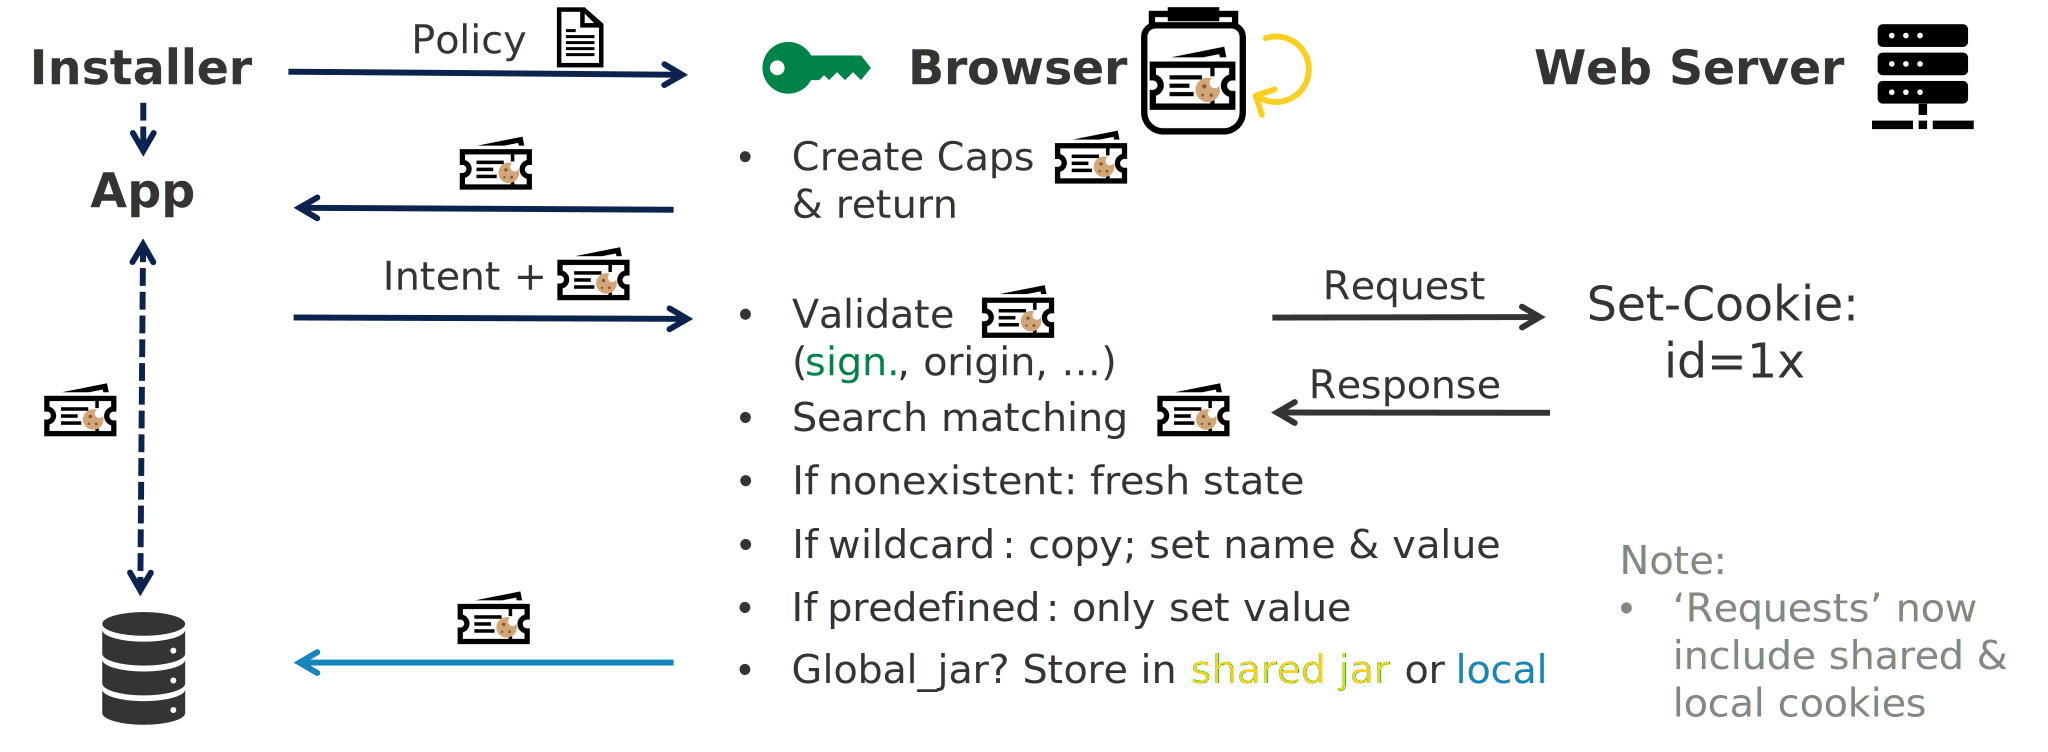
\includegraphics[width=0.9\textwidth]{ByeTrack_Flow.pdf}
%  \caption{}
%  \label{fig:byetrack_overview}
%\end{figure}

Next to performing standard application installations, our custom installer is responsible for extracting each app's policy file and delivering it to the browser for token generation.
To simplify deployment, the apps to be installed are bundled with the installer itself as APK files stored under its \texttt{assets/} directory.
Alternative locations such as the \texttt{res/} folder are unsuitable, as resources are compiled into a binary format that cannot be directly accessed at runtime.
Hosting the APKs remotely and downloading them on demand would also have been possible, but this would introduce unnecessary network dependencies and complicate reproducibility for our proof-of-concept.

Because the assets directory is read-only at runtime, each APK must first be copied into the installer's private file storage before it can be installed.
The installation is then triggered by constructing an explicit Intent ~\cite{android:intent} that references the local file's Uri ~\cite{android:uri}, sets its MIME type to
\texttt{application/vnd.android.package-archive} \cite{android:intent.setdataandtype}, and grants temporary read permissions via \texttt{Intent.FLAG\_GRANT\_READ\_URI\_PERMISSION}.
This intent is launched through a custom ActivityResultLauncher ~\cite{android:activityresultlauncher}, which encapsulates Android's modern
\texttt{ActivityResultContracts.StartActivityForResult} ~\cite{android:activityresultcontracts.startactivityforresult} mechanism.

This construct allows the installer to be notified directly when the installation flow finishes, without requiring any form of polling or background monitoring.
Upon receiving a successful result code, the installer immediately proceeds to locate and read the policy file contained within the newly installed app's assets directory, using Android's \texttt{AssetManager} ~\cite{android:assetmanager}.
The extracted JSON policy is parsed and forwarded to the browser, together with the app's package name and version information obtained via the \texttt{PackageManager} ~\cite{android:packagemanager}.
For this to work, the package names of the apps to be installed must be registered in the Android Manifest under the \texttt{queries} element ~\cite{android:manifest.queries}. 

For inter-process communication, we employ a ContentProvider ~\cite{android:contentprovider} exposed by the browser.
This IPC mechanism was chosen because it offers a straightforward implementation, automatically conveys the caller's UID (enabling reliable authentication of the requesting app), and supports structured data transfer via Bundle objects ~\cite{android:bundle}.

Although Android provides functionality to determine the sender of a broadcast intent since API level 34 ~\cite{android:getsentfrompackage}, we found these to be unreliable in practice -- returning null for dynamically sent intents in our case.
Using a \texttt{PendingIntent} ~\cite{android:pendingintent} as a workaround would still be susceptible to spoofing, since a malicious app could craft and dispatch its own fake pending intent.
A bound service ~\cite{android:boundservice} could also have served as a communication channel but would require the browser process to be running at the time of transmission and would considerably increase implementation complexity.
Thus, the content provider offered the most reliable and maintainable IPC solution for pushing the applications policy file to the browser.

\section{Browser (Fenix)}
The browser serves as the policy enforcement point in our architecture. 
Its modifications fall into two main categories:
(1) token generation and transmitting in \texttt{GeckoView} -- Mozilla's WebView like Java library for Android that exposes the Gecko engine's functionality --, and
(2) the actual cookie enforcement within the C++ back-end of \texttt{Gecko} -- the engine that powers the web browser ~\cite{firefox:frontbackend, firefox:gecko}.

This separation maintains a clear trust boundary between high-level policy logic and low-level enforcement. 
Although their responsibilities overlap conceptually -- especially cryptographic operations on the tokens -- , direct invocation across these layers proved impractical, despite the possibility for \texttt{GeckoView} code to communicate between Java and C++ via the Java Native Interface (JNI) ~\cite{firefox:jni} (see \autoref{subsec:jni_bridging}).

\subsection{Token Generation}
\label{subsec:token_generation}

% --------------------------------Table----------------------------

\begin{table}[h]
\centering
\begin{threeparttable}

\begin{tabular}{@{}lll @{}}

\toprule
Global & Private & Allowed \\ 
\midrule
predefined & wildcard & \checkmark \\
wildcard & wildcard & $\times$ (take private) \\
wildcard & predefined & \checkmark \\
predefined & predefined & $\times$ (take private)\tnote{1} \\
\bottomrule
\end{tabular}

\begin{tablenotes}
  \item[1] \textit{Note: Conflict if domain and cookie name match.}
\end{tablenotes}

\end{threeparttable}
\caption{Allowed combinations of global and private policy entries}
\label{tab:policy-downgrade}
\end{table}

% ---------------------------------------------

Before generating any capability tokens, the browser performs a policy downgrade step to sanitize the received policy (\autoref{tab:policy-downgrade}).
This step ensures that conflicting or overlapping entries are resolved according to the principle of least privilige (PoLP): private entries always take precedence over their global counterpart.

When the content provider receives a policy from the installer, it first parses the JSON structure into four collections directly corresponding to the four sections of the policy: predefined global, predefined private, wildcard global, and wildcard private.
Each collection represents either a mapping from domains to explicit cookie names (for predefined entries), or a list of domains (for wildcard entries).

\textbf{Predefined Conflict Detection:} The first downgrade check handles domain-level and cookie-level conflicts within predefined entries.
If a domain appears in both predefined global and predefined private, the global entry is removed entirely.
If the same cookie name is found under both sections for the same domain, the global cookie is removed, keeping only the private one.
This logic is realized by iterating over the global map and comparing it to the private map and similarly for cookie-level checks.

\textbf{Wildcard Conflict Detection:} A similar check is applied to wildcard entries.
If the same domain appears in both wildcard global and wildcard private, the global entry is discarded.

\textbf{Independence Between Predefined and Wildcard Sections:} 
Importantly, predefined and wildcard rules are treated independently.
The downgrade logic explicitly avoids removing entries across these two categories.
This means that a domain can safely appear in both sections with different privilege levels. 
This independence is reflected in the implementation by simply skipping cross-type downgrades
An example can be found in \autoref{appendix:policy}.

% Actual Generation Part
Once all conflicts are resolved, the downgraded policy structures are passed into the token generation routines -- processing of the predefined map and wildcard list.
These functions iterate over the filtered domain and cookie lists, creating one encrypted capability token per entry using \textsc{generateSingleToken(domain, cookieName, "*", globalJar, packageName, versionName, rights)}.
As a result, only conflict-free and least-privilege token objects of the format described in \autoref{sec:token} are generated:

Note that the classic wildcard tokens omit the \texttt{cookie\_name} and \texttt{cookie\_value} fields, using \texttt{"*"} as placeholder value to indicate that they apply to all cookies for the given domain.
Ambient tokens extend this paradigm further by also omitting the \texttt{domain} field, effectively applying to all domains.
For wildcard tokens, the rights filed is set to \texttt{NONE} by default.
This is due to the reason that wildcard tokens stay the way they are and are used as a blueprint for the browser to generate final tokens when cookies are actually received from the network and hence we do not want developers to accidentally overwrite the cookie value and thereby break the system.

Each token object is then encoded as a compact JSON object and serialized into a Base64-encoded string.
Finally, the encoded string is signed using hmacSHA256 and the signature attached to the token object separated with a dot, similar to JWTs ~\cite{rfc7519}, before encrypting it using AES-CBC with a random IV using the browsers secret key.
This makes the tokens tamper-evident and ensures that only the browser can generate valid tokens.

Once generated, tokens are send to the app in a map from domain to the String representation of the JSON array via the same content provider that received the policy so that the app can persist them locally (\autoref{sec:byetracklib}).

\subsection{Launching Custom Tabs \& TWAs with Tokens}
The browser performs this process in two stages: (1) threading capability data from the Android layer down into the Gecko engine, and (2) enforcing cookie isolation inside Gecko's networking stack.

\paragraph{Stage 1 – Threading of Capability Data.}
The threading mechanism ensures that all capability-related data (tokens and caller information) are propagated consistently through the Android and GeckoView layers until they reach the browser engine.

In Fenix, all incoming intents that trigger a custom tab launch are handled by the \texttt{CustomTabsIntentProcessor} class, which resides in the Android Components library -- Mozilla's reusable collection of browser building blocks.
Since Fenix currently does not support Trusted Web Activities (TWAs), any incoming TWA intent is downgraded to a standard custom tab intent and hence handled by the same processor.

Analogous to the existing \textsc{getAdditionalHeaders()} function -- used to retrieve and attach custom HTTP headers to CT or TWA requests -- we introduce a dedicated function that collects and returns all Byetrack-specific context data.
This function retrieves the final and wildcard capability tokens, the UID of the calling application, a boolean flag and returns them as a structured map.
We need the flag to distinguish between normal website launches initiated by the user and launches initiated by an app via Custom Tabs or TWAs, as only the latter should enforce Byetrack logic.
Otherwise, the normal browsing experience would be affected as no cookies would be stored for normal website visits as the browser would not receive any tokens, and hence drop all cookies.

This map is then threaded through several layers of the Android Components architecture.
Starting from the initial intent processing, it follows the custom tab launch path until it reaches the \texttt{GeckoEngineSession} class.
GeckoEngineSession acts as a bridge between Android Components (where the Custom Tabs logic resides) and GeckoView, Mozilla's Android library that exposes the Gecko browser engine APIs.

Within \texttt{GeckoEngineSession}, the data are handed over to the \texttt{GeckoSession} loader -- the central entry point responsible for initiating page loads in GeckoView.
Here, similar to other loaders that handle fields such as headerFilter, additionalHeaders, or flags, we introduced a new loader to transmit the capability tokens and UID.

Inside this loader, the PackageManager is used to derive the calling app's package name and version name from the UID passed in the intent.
All these values -- tokens, package name, and version name -- are then encapsulated in a \texttt{GeckoBundle}, a lightweight key-value store optimized for inter-process communication between the Java and C++ layers of GeckoView.

The bundle is stored in the \texttt{GeckoSession} and attached to the LoadUri dispatch message.
When this message is processed, the loader extracts the previously stored Byetrack fields and forwards them to the browser's \textsc{fixupAndLoadURIString} function.
The parameters of this function are registered in the \texttt{LoadURIOptions} dictionary which holds load arguments for \texttt{docshell} loads.
The docshell load parameters are initialized in the \texttt{DocShellLoadState} structure and carries functionality to get and set various load options we use in the Gecko's \texttt{DocumentLoadListener}.

Gecko's \texttt{DocumentLoadListener} is responsible for managing the lifecycle of document loads, and therefore the ideal place to give the threaded opaque data meaning by parsing them back into usable tokens.

During the document loading process, the Byetrack integration hooks into the \texttt{DocumentLoadListener} to process and apply capability tokens associated with a given navigation.
The first step is carried out by the function \textsc{ProcessTokenBlob}, which transforms an incoming serialized token blob into validated ByetrackToken objects.
Each blob is first parsed into its individual encrypted token strings, which are then decrypted into their JSON form.
These JSON representations are deserialized into structured token objects and subsequently validated against the current application identity, consisting of the package name and app version.
Tokens that fail to meet these validation criteria are discarded, ensuring that only authentic and context-appropriate capability tokens are propagated further in the loading process.

We implement a \textsc{ApplyByetrackFromLoadStateToBrowserContext} function that transfers our tokens from the \texttt{DocShellLoadState} into the active top level browsing context, where they become accessible thoughout the browsing sessions lifecycle.

The function first verifies that no tokens or cookie headers have already been attached to the context, preventing redundant state updates.
It then retrieves both the final and wildcard token blobs, along with the domain and package metadata, and processes them through the same parsing and validation pipeline.
The final tokens are converted into a consolidated cookie header string, which is attached to the top level browsing context to be used by the network stack during request creation.
Wildcard tokens, on the other hand, are stored directly in the context's internal token array, allowing them to be evaluated dynamically for future requests.

Through this mechanism, the top level browsing context becomes the authoritative holder of Byetrack state for each navigation.
It provides the cookie and network layers with all validated tokens and associated headers needed to enforce domain-scoped tracking policies.
This design ensures that token verification occurs early in the navigation lifecycle while such that they only have to be parsed and validated once per navigation.
This establishes a separation between token management and enforcement, allowing the network layer to focus solely on isolating cookies based on the pre-validated tokens.

\paragraph{Stage 2 – Enforcement of Cookie Isolation.}
The actual enforcement of cookie isolation based on the capability tokens occurs in \texttt{Gecko}'s networking component \textit{Necko} ~\cite{firefox:networking-wiki, firefox:networking-docs}, especially in its \texttt{CookieService} and \texttt{HttpBaseChannel}.
When a network request is initiated, the \texttt{HttpBaseChannel} uses the \texttt{CookieService} to (1) prepare the cookie header for outgoing requests and (2) process incoming Set-Cookie headers from server responses and storing the cookies in the browser storage.

%(HttpBaseChannel::AddCookiesToRequest calls CookieService::GetCookieStringFromHttp & HttpBaseChannel::SetCookieHeaders calls CookieService::SetCookieStringFromHttp are the two functions responsible for these tasks, respectively.)
\paragraph{Outgoing Cookies.}
The main flow for attaching cookies to outgoing requests occurs in \texttt{HttpBaseChannel}'s \textsc{AddCookiesToRequest}.
Here, the \texttt{CookieService}'s  GetCookieStringFromHttp function is called to retrieve the appropriate cookies for the target domain.
Similarly, we use the top-level browsing context to retrieve our prebuilt cookie header string based on the final capabilities associated during the document load phase.
The outgoing request header is constructed by appending our capability-based cookie string to the existing Cookie header, separated by a semicolon.

\paragraph{Incoming Cookies.}
For incoming Set-Cookie headers, \texttt{HttpBaseChannel}'s \textsc{SetCookieHeaders} processes and stores cookies received from server responses.
It calls \textsc{SetCookieStringFromHttp} defined in \texttt{CookieService} iteratively for each cookie string and stores them in the browser's cookie jar.
Here, we again leverage the top-level browsing context to retrieve wildcard capability tokens such as the "\texttt{enforcement}" flag and pass them as an additional parameter.
This location also hosts the CHIPS~\cite{googlechips} implementation, making it straightforward to integrate our logic: CHIPS is evaluated first, and only if it allows storage does the Byetrack logic apply next.

When a response containing cookies is received, our implementation first extracts the cookie name and value from the \texttt{nsCookie} object and logs this information alongside the associated base domain and the number of active tokens currently available for that site.
These tokens represent the capability-based permissions granted to the application according to its installed policy, such as whether specific domains or cookies may be stored globally or privately.

The extracted information is then passed to the function \textsc{DecideCookieAction()}, which encapsulates the core of our decision-making logic.
Before any evaluation occurs, the function checks the \texttt{enforcement} flag to infer whether the \texttt{LoadURI} event of the current session stems from a custom tab launch or from opening a tab normally via the browser.
Depending on this, our enforcement is either enabled or disabled.
In case it disabled, the function immediately returns a decision to store the cookie normally, preserving default browser behavior.
Otherwise, all available tokens for the current cookie are evaluated based on the following precedence rules:

\begin{enumerate}
  \item 
Predefined tokens have absolute priority over wildcard tokens.

  \item
Within the same class, private tokens override global ones, ensuring that stricter privacy rules are always applied when present.

  \item
Wildcard tokens apply when no predefined token is available and indicate that all cookies from that domain should be handled according to their declared scope (global or private).
\end{enumerate}

The result is a \texttt{ByetrackCookieDecision} object that specifies both the action to take (e.g., store, capture, or reject) and the corresponding token that granted the decision.
Depending on this decision, the integration proceeds as follows:

\begin{enumerate}
  \item 
    \textbf{StoreNormally:}
    If the cookie is authorized for global storage (e.g., by a predefined or wildcard global token), Byetrack simply continues the native Gecko cookie insertion flow conducted by \textsc{storage->AddCookie()}.
This preserves default browser functionality for legitimate cases, such as cookies essential for same-site sessions or user preferences.

  \item
    \textbf{CapturePredefined:}
For cookies explicitly defined in the policy as private (e.g., session identifiers that must not leak cross-site), the cookie's value is embedded into the associated token by updating the token's value field.
The token's access rights are updated to \texttt{READ\_WRITE}, reflecting that it now carries an active cookie value -- essentially turning it into a final token.
We do this for the reason how the additional utility on our tokens work (\autoref{sec:utility}).
Instead of being stored in the browser's global jar, this updated token is forwarded to \textsc{StageTokenForReturn()}, a helper routine that serializes the token information and stages it for return to the application the CT launch originated from.

  \item
    \textbf{CaptureWildcard:}
Wildcard tokens behave similarly: if a domain is destined for the private jar by a wildcard rule, not only the cookie name but also the value is captured into the token.
The only important difference is that here, the token's access rights are not updated (default is no access rights \texttt{NONE}), as otherwise the tracking library could simply read out the value again, echo it back to its server, and thereby circumvent our cookie-isolation.

  \item
    \textbf{Reject:}
If no token matches the cookie or if the policy forbids storing cookies for this domain, the cookie is dropped.
This prevents unwanted cross-site tracking by suppressing unauthorized cookie storage operations.

\end{enumerate}

This ensures that all unmodified web behavior remains intact while Byetrack enforces policy-based restrictions transparently.

\paragraph{Returning Tokens to the App} 
\label{par:returning_tokens}

Before the token is serialized again and handed back up to the java layer to be sent to the app, we need to make sure that the token does not already exist in the app's private jar.
For this, we fetch the cookie header stored in the top level browsing context and check if the cookie encapsulated by the token is already present in the header.
This is done by re-constructing the standard cookie representation "\texttt{token.name}=\texttt{token.value}" and checking if it is contained in the merged cookie header stored in the top level browsing context, used for outgoing requests.
Note, that for simplictly we only consider the standard cookie representation here and do not check for additional attributes such as \texttt{Path}, \texttt{Domain}, or \texttt{Secure}, which could be added in a more advanced implementation \autoref{chap:future_work}.
If the token is found there, we discard it as the app already stores it in its private jar and there is no need to return it again.
Otherwise, the token payload is serialized back into its JSON representation and then Base64-encoded, signed and encrypted the same way as during generation, before it is added to a temporary map stored in the \texttt{HttpBaseChannel} object by using its internal channel.
This map associates each domain with an array of token strings, allowing multiple tokens for different domains to be staged for return to the application.

To synchronize the browser's enforcement results with the application process, we extends \texttt{Gecko}'s networking stack with a dedicated emission helper implemented in \texttt{HttpBaseChannel}'s \textsc{EmitByetrackTokensToGeckoView()}.
This function is invoked from \texttt{HttpChannelParent}'s \textsc{OnStopRequest()} -- that is, at the exact moment when an HTTP request completes and all cookies have been processed by the \texttt{CookieService}.
Note that at this point, our subsystem has already collected any filled in tokens tokens into the temporary map stored in the channel object by the \textsc{StageTokenForReturn()} function.

The \textsc{EmitByetrackTokensToGeckoView()} helper serializes this in-memory map into a compact JSON structure and forwards it through \texttt{Gecko}'s observer service.
Before emitting, the function checks a boolean flag and a unique batch identifier to prevent re-emitting the same batch of tokens multiple times for a single channel instance.
Using mozillas JSON writer utility, the function iterate voer the map entries, associating each domain with an array of token strings.
The output of the JSON follows the same structure as the one used during token generation, ensuring consistency between the two processes and thereby simplifying parsing on the receiving end.
The function uses the global \texttt{nsIObserverService} to broadcast a notification with the topic "byetrack-final-tokens".
This effectively acts as an IPC bridge between the networking layer in C++ and JavaScript/Java.
After emitting the tokens, the internal map is cleared to avoid redundant emissions.

By performing this emission inside \texttt{HttpChannelParent}'s \textsc{OnStopRequest()}, we guarantee that the final set of captured tokens is only emitted once the HTTP transaction has completed and all cookies have been processed.
This ensures that no partial or intermediate state is sent to the embedding application.

On the embedding side, the "byetrack-final-tokens" observer event is handled within \texttt{GeckoViewNavigation}, the same place where the threading in \texttt{GeckoView} started.
The observer's \textsc{observe()} method processes the serialized JSON map and uses \texttt{GeckoView}'s event dispatch system to send a message of type "GeckoView:Byetrack:FinalTokens" carrying the tokens and the application identity (package name).
This event is caught on the Java side inside the responsible \texttt{GeckoSession} -- the same locaiton where LoadUri and similar events are processed.
When the "GeckoView:Byetrack:FinalTokens" event is received, the Java handler constructs a \texttt{ContentValues} ~\cite{android:contentvalues} object containng the token JSON and writes it to the application's registered \texttt{ContentProvider} ~\cite{android:contentprovider}, allowing it to update its local capability store.


\subsection{Additional Utility}
\label{sec:utility}

All additional utility functions are implemented in a separate \texttt{ContentProvider} ~\cite{android:contentprovider} exposed by the browser.
In this content provider, we leverage the parameter "method" of the \textsc{call} function ~\cite{android:contentprovider:call} to distinguish between the different utility functions.
This also implies that all results are returned as a Bundle object, which is the standard return type of the call function.
The data for each function to work on is passed via remaining parameters of the function -- \textsc{arg} (String) and \textsc{extras} (Bundle) if necessary. 

\paragraph{GetTokenNames.} 
If the method parameter is set to \texttt{"get\_token\_cookie\_names"}, the function expects a list of capability tokens in JSON array format as the \textsc{arg} parameter.
Each token is decoded from its encrypted form using the \texttt{Token.decodeEncrypted()} function, which reconstructs the underlying \texttt{TokenPayload}.
If the decoded token's \texttt{applicationId} does not match the caller's package name, the request is rejected.
Otherwise, the function adds the mapping between the token string and its associated cookie name to the resulting \texttt{Bundle}, which is then returned to the caller.
This enables external applications (e.g., the Byetrack client library) to inspect which cookie names are encapsulated by their issued capability tokens, without disclosing data from other apps.

\paragraph{GetTokenValue.}
If the method parameter is set to \texttt{"get\_token\_cookie\_value"}, the function expects a single encrypted capability token as the \textsc{arg} parameter.
Similar to the previous case, the token is decoded and verified against the caller's package name.
Afterwards, the browser verifies the access rights encoded within the capability token.
Only if the \textsc{canRead()} flag inside the payload is set does the provider return the corresponding cookie value as the field \texttt{"value"} in the result \texttt{Bundle}.
Otherwise, a permission error string is returned.
This design enforces read isolation and ensures that only apps possessing valid read rights for a specific capability can query associated cookie values.

\paragraph{WriteTokenValue.}
If the method parameter is set to \texttt{"write\_token\_cookie\_value"}, the provider allows controlled modification of the cookie value embedded in a capability token.
Again, the encrypted token is decoded, verified against the caller's package name, and its permissions checked via \textsc{canWrite()}.
If write access is permitted, the new cookie value is taken from the \textsc{extras} bundle under the key \texttt{"value"}.
Since all fields of the payload are immutable, a new \texttt{TokenPayload} instance is created internally with the updated value, re-signed using the browser's signing key, and re-encrypted into a new token string.
The updated token and its target domain are then returned to the caller.
This process ensures that all token modifications remain cryptographically verifiable and bound to the correct application context.

\section{App-side Integration}
\label{sec:appside}

On the application side, we introduced two main components to enable seamless integration of Byetrack into existing Android apps:
(1) a standalone Byetrack helper library that encapsulates capability token management, and 
(2) a customized AndroidX Browser library that automatically injects tokens into all CT and TWA launches.
Together, these components ensure that apps using standard AndroidX interfaces transparently benefit from Byetrack's protection without code modifications.

\subsection{Byetrack Helper Library}
\label{sec:byetracklib}

The Byetrack library acts as the bridge between the embedding app and the browser.
It manages the storage, retrieval, and injection of capability tokens and exposes a minimal, high-level API through the \texttt{ByetrackClient} class.
Internally, it consists of several modular components that collectively handle token management, secure communication with the browser, and intent preparation.

\paragraph{Token Management.}
To facilitate secure and persistent token handling, the library exposes a \texttt{ContentProvider} (\texttt{TokenProvider}) through which the browser can deliver tokens to the application.
This provider only implements the \textsc{insert()} ~\cite{android:contentprovider:insert} method, as neither querying nor deletion is required.
When the browser calls \textsc{insert()}, the library first verifies the calling package name to ensure that only legitimate browsers can write to the app's token store.
Upon successful verification, the transmitted tokens -- typically provided as a key-value map containing both final and wildcard tokens -- are persisted locally.

Tokens are stored in \texttt{SharedPreferences} ~\cite{android:sharedpreferences} under separate namespaces -- \texttt{final\_token}, \texttt{wildcard\_token}, and \texttt{is\_ambient} -- to distinguish between different token types.
The additional ambient flag indicates whether the app is currently operating in "ambient mode", which is crucial for correctly interpreting tokens that otherwise share the same structure.

\texttt{SharedPreferences} were chosen for simplicity, persistence across restarts, and asynchronous write support -- characteristics well suited for our lightweight storage requirements.
The \texttt{TokenManager} class abstracts all access to this local storage, offering thread-safe read and write operations and providing convenience wrappers to fetch or update specific token sets.

\paragraph{Token Injection into Intents.}
Before launching a browser instance, the app must attach its capability tokens to the outgoing intent.
This is handled by the \texttt{ByetrackClient} via its \textsc{attachTokens()} and \textsc{injectTokens()} methods.
When called, these methods gather all relevant tokens from the store, serialize them into a compact JSON bundle, and append them to the intent extras.
If additional domains are supplied, the function ensures that the respective tokens are also included.

This injection step is completely transparent to the embedding app.
Developers can use the same convenient methods \textsc{launchUrl()} ~\cite{android:customtabsintent:launchurl} and \textsc{launchTrustedWebActivity()} ~\cite{android:trustedwebactivityintent:launchtrustedwebactivity} for launching a custom tabs intent and trusted web activity intent as before; the library automatically enriches them with the necessary Byetrack metadata prior to launch.

\paragraph{Utility Components.}
Supporting utilities such as \texttt{Util} and \texttt{DebugHelp} provide helper functions for (1) calling the browser's exposed content provider for additional operations on tokens and (2) displaying debug information about the current token stored and which cookies they encapsulate.
%These are deliberately kept separate from the core logic, but can easily be imported and used by the embedding app.

\subsection{AndroidX Browser Integration}
\label{sec:androidx-browser}

\begin{figure}[h]
  \lstinputlisting[language=Java]{~/Projects/thesis_repos/thesis/thesis-template/res/code/launchUrl.java}
  \caption{Token injection in Custom Tabs launch function}
  \label{code:customtablaunch}
\end{figure}

To eliminate the need for developers to manually include the Byetrack library or modify their own app code, we integrated it directly into a fork of the \texttt{AndroidX Browser} library ~\cite{android:androidxbrowser}.
This ensures automatic token injection whenever an app uses CTs or TWAs.

Specifically, both \texttt{CustomTabsIntent}'s \textsc{launchUrl()} and \texttt{TrustedWebActivityIntent}'s \textsc{launchTrustedWebActivity()} were extended to call the \textsc{attachTokens()} method of the exposed client before invoking the activity. 
This guarantees that every navigation initiated through these standard \texttt{AndroidX} interfaces automatically carries the appropriate capability tokens to the browser.

Additionally, we introduced overloaded versions of both launch functions that accept an optional list of additional hosts.
These allow developers to specify related domains that should receive tokens as well -- for instance, if the application anticipates cross-domain requests as part of the same trust context.

Overall, these modifications make Byetrack entirely transparent to app developers: any app compiled against our customized \texttt{AndroidX Browser} version inherently benefits from Byetrack's mitigation without requiring code changes or awareness of the underlying token system.

\section{Integration into Existing HyTrack Demo Applications}
\label{sec:hytrackapps}

Both HyTrack demo applications, \texttt{CrossAppLauncher} and \texttt{CrossAppTrackerOne}, originally launched Trusted Web Activities (TWAs) using Chrome's \texttt{android-browser-helper} library ~\cite{chrome:androidbrowserhelper}, which automatically establishes a TWA connection to Chrome for convenience.
To make these apps compatible with our mitigation system, we removed this dependency and integrated our modified \texttt{AndroidX Browser} library instead.
The TWA connection is now established manually with our customized Fenix browser.

For the launcher variant, we additionally implemented a standalone \texttt{TwaLauncherActivity} that launches a TWA on startup, since Firefox currently does not provide a comparable helper library like Chrome does.
Although Firefox does not natively support TWAs yet, no further changes to the applications were required: the TWA intents are transparently downgraded to standard Custom Tab intents within the browser.

\section{Implementation Challenges}
\label{sec:implementation_challenges}

The implementation process presented several notable challenges that required balancing security, practicality, and compatibility with existing Android mechanisms. 
This section summarizes the most critical ones encountered during development.

\subsection{Securely Identifying the Calling Application}

The most crucial challenge was securely identifying the application that launched a Custom Tab.  
This information is essential to verify that the capability tokens presented to the browser genuinely belong to the invoking application and are not spoofed by another app.  
In contrast, Trusted Web Activities are not affected by this problem, as by design, they require a session with the browser over a Binder channel that inherently conveys the caller's identity.

Although Android's \texttt{Intent} mechanism provides an IPC channel between applications, it does not include a built-in way to authenticate the sender of an intent.  
We therefore explored multiple approaches to securely determine the calling application's identity, many of which turned out to be insecure or impractical within our threat model (see ~\autoref{sec:threat_model}).

\paragraph{Plain Intent Extras.}
The simplest approach was to attach the application's package name as an extra to the intent, similar to how capability tokens are passed.  
However, this method is fundamentally insecure since the package name is merely a string that can easily be spoofed by a malicious app pretending to be another package.
Consequently, the malicious app could launch a Custom Tab with tokens belonging to the legitimate app, thereby bypassing our protections.

\paragraph{Shared Secret and Challenge-Response.}
A more advanced approach was to establish a shared secret between the application and the browser (e.g., using the \texttt{KeyStore}) and perform a challenge–response protocol during Custom Tab launch.  
This approach fails under our threat model, since a tracking library included in the app has the same privileges as the app itself and can therefore access the shared secret and execute the challenge–response on its own.  
Consequently, this mechanism cannot prevent colluding apps or libraries from impersonating the legitimate caller.

\paragraph{Using a Medium that Provides Caller Identity.}
We also explored mechanisms that inherently expose the caller's identity to the browser, such as using a Binder-based communication channel.  
However, deriving the identity from such a medium and linking it securely to the Custom Tab launch intent proved difficult, as any identifier accessible to the app is also accessible to the tracking library, and can thus be spoofed.

\paragraph{Commitment Scheme.}
\label{par:commitment_scheme}
Inspired by cryptographic commitment schemes ~\cite{enwiki:1318450859}, we considered a two-phase protocol involving a \emph{commit} and a \emph{reveal} phase.  
In this design, the application would first commit the intended URL and capability tokens via a secure channel from which the browser can derive the caller's identity.  
When the Custom Tab is later launched, the intent itself remains empty, and the browser uses the previously committed data.  

While this design provides strong authenticity guarantees -- since the commitment occurs over a secure channel -- it introduces significant complexity.  
The app must perform two separate actions (commit and reveal), and any other app could trigger a launch using previously committed data, as there is no strong link between the two phases.

\paragraph{Pending Intent.}
\label{par:pending_intent}
A more practical alternative was to leverage Android's \texttt{PendingIntent} mechanism~\cite{android:pendingintent}.  
In this approach, the intent originally used to launch the Custom Tab is wrapped into a \texttt{PendingIntent} flagged as immutable, and capability tokens are attached as extras.  
The browser can then obtain the caller identity securely via \textsc{getCreatorPackage()} or \textsc{getCreatorUid()} and invoke the \texttt{PendingIntent} on behalf of the app.  
Even if another app gains access to this \texttt{PendingIntent}, it cannot alter its content or spoof the original app's identity.  
This method therefore provides a viable balance between security and usability

\paragraph{TWA-like Launch Modifications.}
\label{par:modifying_ct_launch}
Another potential approach was to redesign the Custom Tab launch mechanism to more closely resemble the session-based launch flow used by Trusted Web Activities (TWAs).
In a TWA launch, the application must first bind to the browser's \texttt{CustomTabsService} ~\cite{android:customtabsservice} and establish a verified session.
This binding step inherently conveys the caller's identity to the browser because it relies on an authenticated Binder IPC connection rather than opaque intent extras etc.
Therefore, one possible solution would have been to require all CT launches to follow the same pattern: before opening a URL, the app would be forced to bind to the \texttt{CustomTabsService}, obtain a validated session, and pass that session token to the browser when launching the Custom Tab.

A major downside both the pending intent solution and commitment scheme face is the requirement to modify how Custom Tabs are launched under the hood.
Consequently, our browser modifications are incompatible with existing apps that use the standard \texttt{AndroidX Browser} library for Custom Tab launches, breaking backwards compatibility.

\paragraph{Compatibility Considerations.}
Across all of these alternatives, a common issue emerges: each requires modifying how applications launch Custom Tabs.
Whether through a two-phase commit–reveal sequence, wrapping the launch intent in an immutable \texttt{PendingIntent}, or enforcing a TWA-style session-binding flow, all approaches deviate from the standard \texttt{AndroidX Browser} contract.
As a result, any solution along these lines would break backwards compatibility with existing applications that rely on the conventional intent-based Custom Tab launch mechanism.
For this reason, although these designs provide interesting security properties, they were ultimately not pursued.

\paragraph{Custom Android SDK Extension for Secure Caller Identity Propagation}
To maintain compatibility with existing apps, we ultimately opted for a solution that allows the app to launch Custom Tabs using the standard API while still securely conveying the caller's identity.
While the \texttt{ActivityTaskManagerService} ~\cite{android:activitytaskmanagerservice} internally tracks the calling UID for permission checks and task management, this information is not encoded in the Intent object itself and therefore becomes inaccessible to the receiving application.
To address this, we extended the Android framework with a custom, SDK-level enhancement that embeds the caller's UID directly into the Intent object.
We introduced a new field \texttt{mRealCallingUid} along with a dedicated getter and setter.
To ensure the field survives all typical Intent operations, including activity launches, redirections, and cross-process transmissions, we extended the intents copy-constructor, such as the parcel serialization and deserialization methods to handle this new field appropriately.

The next step was to ensure that the field is populated with the correct value inside the system server.
We extended \texttt{ActivityStarter.startActivityInner()} ~\cite{android:activitystarter}, which is invoked during activity launches after the ActivityManagerServer ~\cite{android:activitymanagerservice} has fully resolved the activity and determined the real calling UID.
Here, the realCallingUid is injected into the intent immediately before the system hands control to the target application (e.g., the browser).
Since the field is part of the intent's serialized state, the target browser process reliably receives it without modification or interference.

This approach provides a trustworthy, non-spoofable channel for conveying the caller's identity to the receiving browser, enabling capability-based cookie isolation without breaking compatibility with existing app behavior.
However, this solution requires applications to compile against our customized Android SDK, since the new accessor for \texttt{mRealCallingUid} is not part of the standard API.
This may limit adoption in practice.
Ideally, Android would natively expose the verified caller identity within \texttt{Intent}, which would eliminate the need for a custom SDK while retaining the security properties demonstrated by our implementation.

\subsection{Bridging Between Java and Native Layers}
\label{subsec:jni_bridging}

In our design, token generation (\autoref{subsec:token_generation}), returning tokens to the app (\autoref{par:returning_tokens}), and querying the browser for additional token-related metadata (\autoref{sec:utility}) are executed entirely within the Java layer, whereas enforcement is implemented inside the C++ network stack.
Both layers require identical utility functions for JSON token parsing, encryption and decryption, and signature generation.
From a software engineering perspective, the ideal architecture would place these utilities exclusively in the C++ layer and expose them to Java via JNI.
This would provide a single source of truth and eliminate code duplication.

GeckoView supports such cross-layer calls through its \texttt{@WrapForNative} annotation, allowing Java code to invoke native C++ functions.
However, these calls require an active \texttt{GeckoRuntime} instance ~\cite{firefox:rni:runtime}.
In our case, token generation and content-provider based utility calls occur before the browser process is fully initialized, meaning no runtime is yet available.
Attempting to temporarily bootstrap a runtime solely for token processing proved unreliable and introduced substantial complexity.

For these reasons, we ultimately separated responsibilities:
the Java layer handles token creation, management, and policy interpretation, while the C++ layer enforces capability constraints once the browser process and its runtime are active.
To maintain secure coordination without requiring direct JNI calls, both layers share a cryptographic secret known only to the browser. This enables the Java layer to prepare signed and encrypted token objects that the C++ enforcement layer can later validate without depending on shared execution context.
